\section{Elementos visuais}\label{RS0001:styles}

Neste guia são listadas possibilidades de apresentação diferenciada e organização da informação nas publicações do portal. Cada uma contém uma imagem com um exemplo do resultado esperado e um trecho de código que deve ser inserido por meio do editor HTML avançado de publicações do portal (ver \cref{RS0001:fig:exemplo-editor}).

\begin{figure}[!ht]
    \centering
    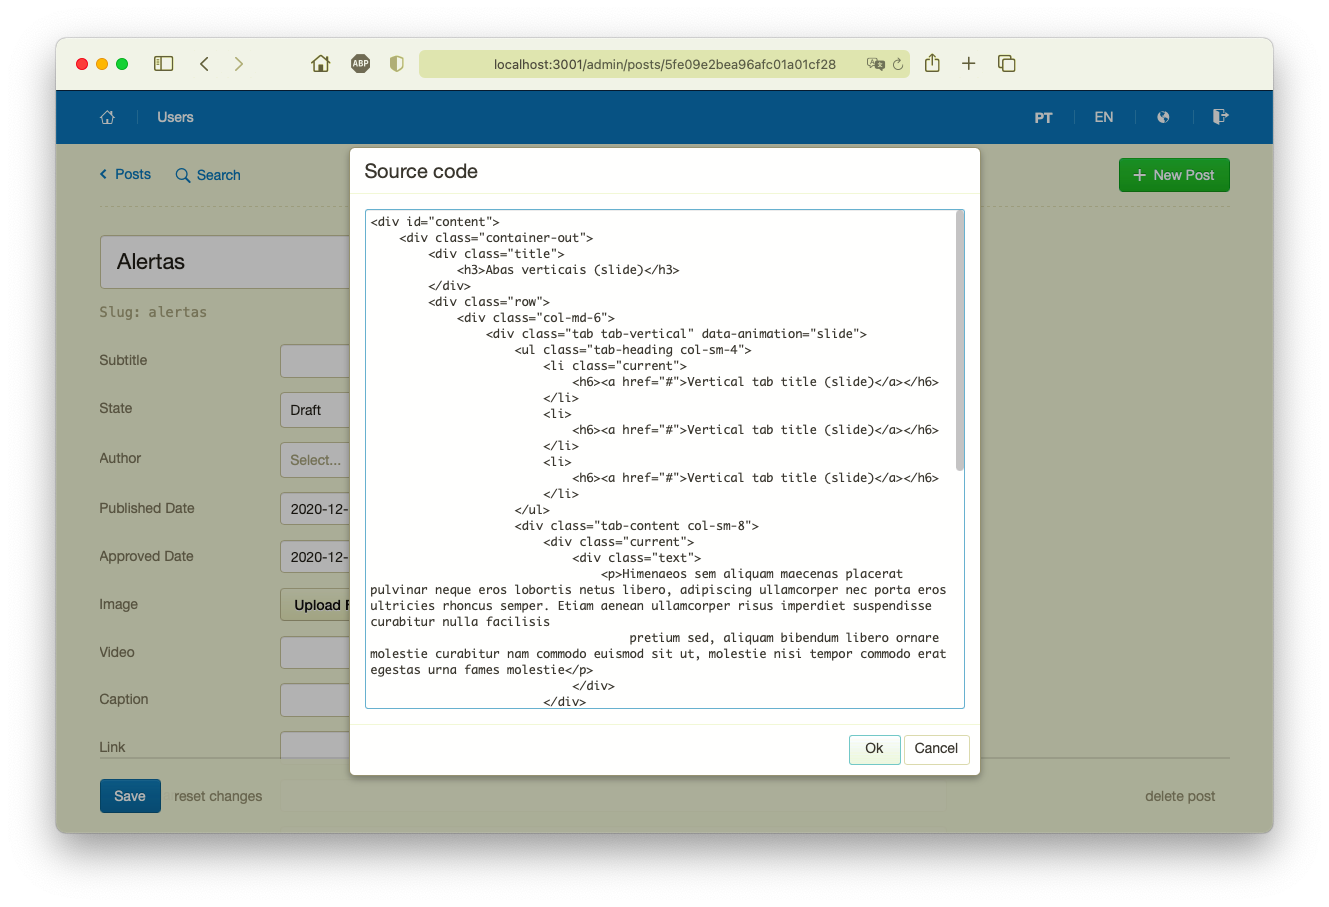
\includegraphics[scale=.25]{exemplo-editor}
    \caption{Exemplo inclusão de texto em destaque no editor HTML avançado}\label{RS0001:fig:exemplo-editor}
\end{figure}

Muitas das opções (as mais utilizadas) listadas neste guia podem ser inseridas por meio do editor \gls{WYSIWYG} (opção ``\textit{Templates}'') e em seguida editadas para atender a necessidade do usuário. Observe porém que muitas das opções mais avançadas não possuem um editor sofisticado (como os de tabelas ou listas por exemplo), e se for necessário inserir ou remover elementos deverá ser utilizado o editor \gls{HTML}.

\subsection{Abas}


\subsubsection{Abas simples}

Organização de texto horizontalmente com foco num tópico por vez.

\begin{figure}[!ht]
    \centering
    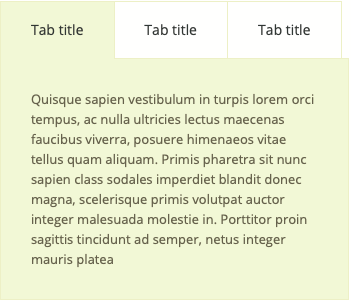
\includegraphics[scale=.5]{abas-simples}
    \caption{Abas simples}\label{RS0001:fig:abas-simples}
\end{figure}

\begin{code}
    \inputminted[label=abas-slide.html]{html}{../RS0001/anexos/abas-simples.html}
    \caption{Exemplo de abas simples}\label{RS0001:code:exemplo-abas-simples}
\end{code}


\subsubsection{Abas (slide)}

Igual à aba simples, porém acrescenta o efeito de deslizamento lateral na mudança de aba. Observe que houve uma quebra de linha nas abas pois os títulos ocuparam um espaço maior que o reservado.

\begin{figure}[!ht]
    \centering
    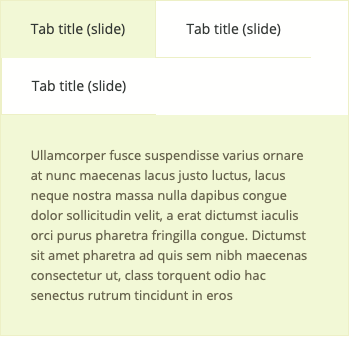
\includegraphics[scale=.5]{abas-slide}
    \caption{Abas (slide)}\label{RS0001:fig:abas-slide}
\end{figure}

\begin{code}
    \inputminted[label=abas-slide.html]{html}{../RS0001/anexos/abas-slide.html}
    \caption{Exemplo de abas (slide)}\label{RS0001:code:exemplo-abas-slide}
\end{code}


\subsubsection{Abas (longas)}

Abas ocupando a largura total da publicação.

\begin{figure}[!ht]
    \centering
    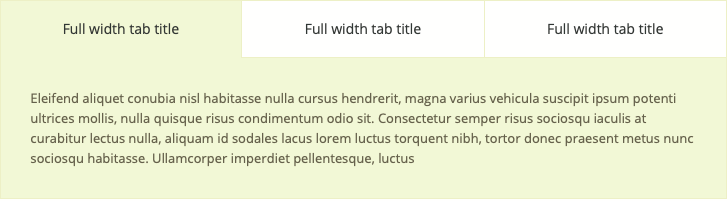
\includegraphics[scale=.5]{abas-longa}
    \caption{Abas (longas)}\label{RS0001:fig:abas-longa}
\end{figure}

\begin{code}
    \inputminted[label=abas-longa.html]{html}{../RS0001/anexos/abas-longa.html}
    \caption{Exemplo de abas (longa)}\label{RS0001:code:exemplo-abas-longa}
\end{code}


\subsubsection{Abas verticais simples}

Organização do texto verticalmente com foco num tópico por vez. Observe que houve uma quebra de linha nas abas pois os títulos ocuparam um espaço maior que o reservado.

\begin{figure}[!ht]
    \centering
    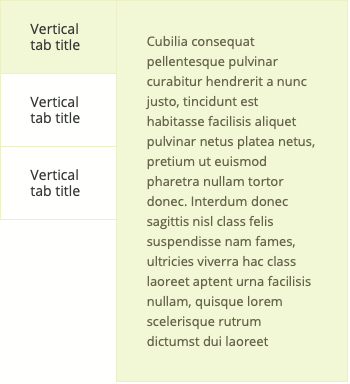
\includegraphics[scale=.5]{abas-vertical-simples}
    \caption{Abas verticais simples}\label{RS0001:fig:abas-vertical-simples}
\end{figure}

\begin{code}
    \inputminted[label=abas-vertical-simples.html]{html}{../RS0001/anexos/abas-vertical-simples.html}
    \caption{Exemplo de abas verticais simples}\label{RS0001:code:exemplo-abas-vertical-simples}
\end{code}


\subsubsection{Abas verticais (slide)}

Igual à aba vertical simples, porém acrescenta o efeito de deslizamento longitudinal na mudança de aba. Observe que houve uma quebra de linha nas abas pois os títulos ocuparam um espaço maior que o reservado.

\begin{figure}[!ht]
    \centering
    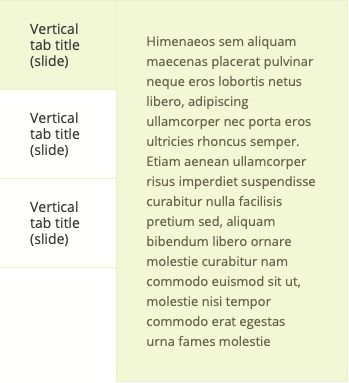
\includegraphics[scale=.5]{abas-vertical-slide}
    \caption{Abas verticais simples (slide)}\label{RS0001:fig:abas-vertical-slide}
\end{figure}

\begin{code}
    \inputminted[label=abas-vertical-slide.html]{html}{../RS0001/anexos/abas-vertical-slide.html}
    \caption{Exemplo de abas verticais (slide)}\label{RS0001:code:exemplo-abas-vertical-slide}
\end{code}


\subsubsection{Abas coloridas simples}

\begin{figure}[!ht]
    \centering
    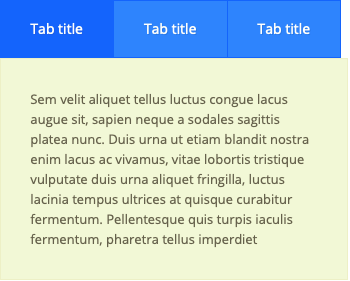
\includegraphics[scale=.5]{abas-coloridas-simples}
    \caption{Abas coloridas simples}\label{RS0001:fig:abas-coloridas-simples}
\end{figure}

\begin{code}
    \inputminted[label=abas-abas-coloridas-simples.html]{html}{../RS0001/anexos/abas-coloridas-simples.html}
    \caption{Exemplo de abas coloridas simples}\label{RS0001:code:exemplo-abas-coloridas-simples}
\end{code}


\subsubsection{Abas coloridas (slide)}

\begin{figure}[!ht]
    \centering
    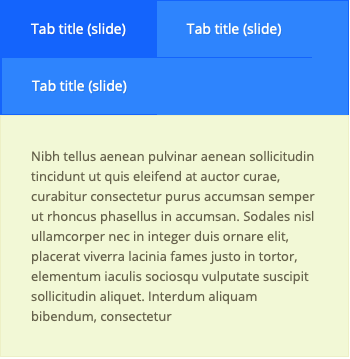
\includegraphics[scale=.5]{abas-coloridas-slide}
    \caption{Abas coloridas (slide)}\label{RS0001:fig:abas-coloridas-slide}
\end{figure}

\begin{code}
    \inputminted[label=abas-abas-coloridas-slide.html]{html}{../RS0001/anexos/abas-coloridas-slide.html}
    \caption{Exemplo de abas coloridas (slide)}\label{RS0001:code:exemplo-abas-coloridas-slide}
\end{code}


\subsubsection{Abas coloridas (longas)}

\begin{figure}[!ht]
    \centering
    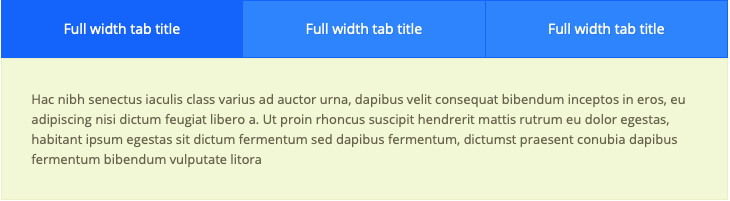
\includegraphics[scale=.5]{abas-coloridas-longa}
    \caption{Abas coloridas (longas)}\label{RS0001:fig:abas-coloridas-longa}
\end{figure}

\begin{code}
    \inputminted[label=abas-abas-coloridas-longa.html]{html}{../RS0001/anexos/abas-coloridas-longa.html}
    \caption{Exemplo de abas coloridas (longas)}\label{RS0001:code:exemplo-abas-coloridas-longa}
\end{code}


\subsubsection{Abas coloridas verticais simples}

\begin{figure}[!ht]
    \centering
    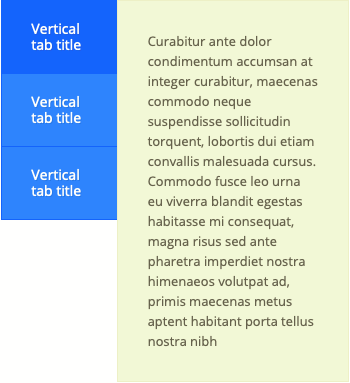
\includegraphics[scale=.5]{abas-coloridas-vertical-simples}
    \caption{Abas coloridas verticais simples}\label{RS0001:fig:abas-coloridas-vertical-simples}
\end{figure}

\begin{code}
    \inputminted[label=abas-abas-coloridas-vertical-simples.html]{html}{../RS0001/anexos/abas-coloridas-vertical-simples.html}
    \caption{Exemplo de abas coloridas verticais simples}\label{RS0001:code:exemplo-abas-coloridas-vertical-simples}
\end{code}


\subsubsection{Abas coloridas verticais (slide)}

\begin{figure}[!ht]
    \centering
    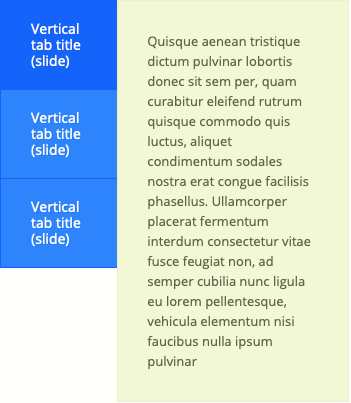
\includegraphics[scale=.5]{abas-coloridas-vertical-slide}
    \caption{Abas coloridas verticais (slide)}\label{RS0001:fig:abas-coloridas-vertical-slide}
\end{figure}

\begin{code}
    \inputminted[label=abas-abas-coloridas-vertical-slide.html]{html}{../RS0001/anexos/abas-coloridas-vertical-slide.html}
    \caption{Exemplo de abas coloridas verticais (slide)}\label{RS0001:code:exemplo-abas-coloridas-vertical-slide}
\end{code}

\subsection{Alertas}

Alertas são utilizados para destacar informações que possuem uma ação simples. A ação pode ser desde o redirecionamento para outra publicação dentro do próprio portal ou para um site externo.


\subsubsection{Chamada simples com botão à esquerda}

\begin{figure}[!ht]
    \centering
    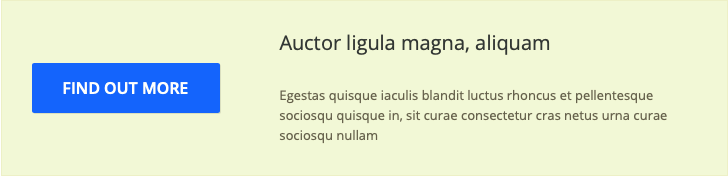
\includegraphics[scale=.5]{chamada-simples-botao-esquerdo}
    \caption{Chamada simples com botão à esquerda}\label{RS0001:fig:chamada-simples-botao-esquerdo}
\end{figure}

\begin{code}
    \inputminted[label=chamada-simples-botao-esquerdo.html]{html}{../RS0001/anexos/chamada-simples-botao-esquerdo.html}
    \caption{Exemplo de chamada simples com botão à esquerda}\label{RS0001:code:exemplo-chamada-simples-botao-esquerdo}
\end{code}


\subsubsection{Chamada simples com botão à direita}

\begin{figure}[!ht]
    \centering
    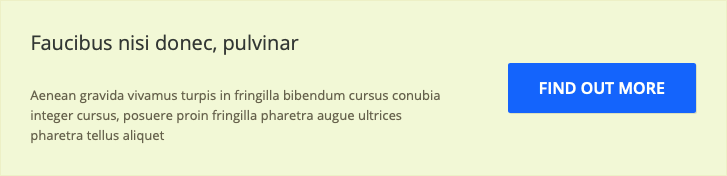
\includegraphics[scale=.5]{chamada-simples-botao-direito}
    \caption{Chamada simples com botão à direita}\label{RS0001:fig:chamada-simples-botao-direito}
\end{figure}

\begin{code}
    \inputminted[label=chamada-simples-botao-direito.html]{html}{../RS0001/anexos/chamada-simples-botao-direito.html}
    \caption{Exemplo de chamada simples com botão à direita}\label{RS0001:code:exemplo-chamada-simples-botao-direito}
\end{code}


\subsubsection{Chamada vertical simples}

\begin{figure}[!ht]
    \centering
    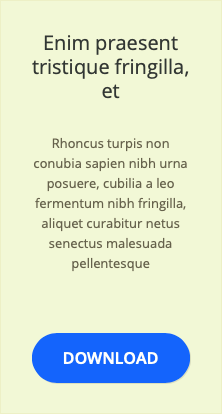
\includegraphics[scale=.5]{chamada-vertical-simples}
    \caption{Chamada vertical simples}\label{RS0001:fig:chamada-vertical-simples}
\end{figure}

\begin{code}
    \inputminted[label=chamada-vertical-simples.html]{html}{../RS0001/anexos/chamada-vertical-simples.html}
    \caption{Exemplo de chamada vertical simples}\label{RS0001:code:exemplo-chamada-vertical-simples}
\end{code}


\subsubsection{Chamada vertical com fundo listrado}

Semelhante à ``Chamada vertical simples'' porém com um fundo listrado.

\begin{figure}[!ht]
    \centering
    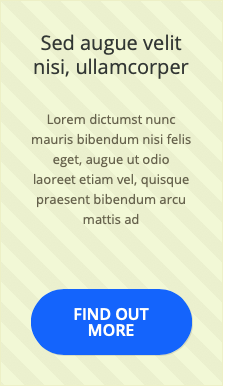
\includegraphics[scale=.5]{chamada-vertical-listrada}
    \caption{Chamada vertical listrada}\label{RS0001:fig:chamada-vertical-listrada}
\end{figure}

\begin{code}
    \inputminted[label=chamada-vertical-listrada.html]{html}{../RS0001/anexos/chamada-vertical-listrada.html}
    \caption{Exemplo de chamada vertical listrada}\label{RS0001:code:exemplo-chamada-vertical-listrada}
\end{code}


\subsubsection{Chamada vertical com fundo listrado dinâmico}

Semelhante à ``Chamada vertical com fundo listrado'' porém o fundo tem um efeito de visual de deslocamento (somente visível numa tela de computador).

\begin{figure}[!ht]
    \centering
    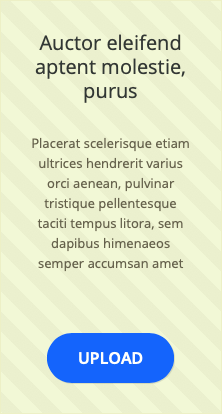
\includegraphics[scale=.5]{chamada-vertical-listrada-animada}
    \caption{Chamada vertical listrada dinâmica}\label{RS0001:fig:chamada-vertical-listrada-animada}
\end{figure}

\begin{code}
    \inputminted[label=chamada-vertical-listrada-animada.html]{html}{../RS0001/anexos/chamada-vertical-listrada-animada.html}
    \caption{Exemplo de chamada vertical listrada dinâmica}\label{RS0001:code:exemplo-chamada-vertical-listrada-animada}
\end{code}


\subsubsection{Chamada colorida com botão à esquerda}

\begin{figure}[!ht]
    \centering
    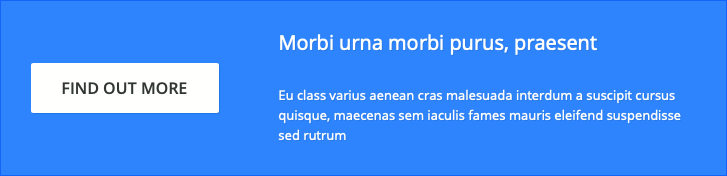
\includegraphics[scale=.5]{chamada-colorida-botao-esquerdo}
    \caption{Chamada colorida com botão à esquerda}\label{RS0001:fig:chamada-colorida-botao-esquerdo}
\end{figure}

\begin{code}
    \inputminted[label=chamada-colorida-botao-esquerdo.html]{html}{../RS0001/anexos/chamada-colorida-botao-esquerdo.html}
    \caption{Exemplo de chamada colorida com botão à esquerda}\label{RS0001:code:exemplo-chamada-colorida-botao-esquerdo}
\end{code}


\subsubsection{Chamada colorida com botão à direita}

\begin{figure}[!ht]
    \centering
    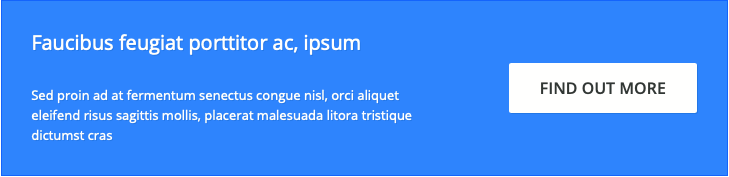
\includegraphics[scale=.5]{chamada-colorida-botao-direito}
    \caption{Chamada colorida com botão à direita}\label{RS0001:fig:chamada-colorida-botao-direito}
\end{figure}

\begin{code}
    \inputminted[label=chamada-colorida-botao-direito.html]{html}{../RS0001/anexos/chamada-colorida-botao-direito.html}
    \caption{Exemplo de chamada colorida com botão à direita}\label{RS0001:code:exemplo-chamada-colorida-botao-direito}
\end{code}


\subsubsection{Chamada vertical colorida}

\begin{figure}[!ht]
    \centering
    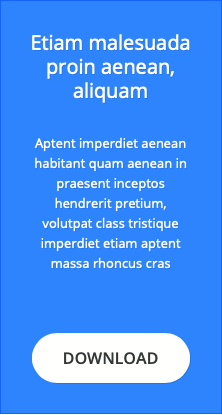
\includegraphics[scale=.5]{chamada-vertical-colorida}
    \caption{Chamada vertical colorida}\label{RS0001:fig:chamada-vertical-colorida}
\end{figure}

\begin{code}
    \inputminted[label=chamada-vertical-colorida.html]{html}{../RS0001/anexos/chamada-vertical-colorida.html}
    \caption{Exemplo de chamada vertical colorida}\label{RS0001:code:exemplo-chamada-vertical-colorida}
\end{code}


\subsubsection{Chamada vertical colorida com fundo listrado}

\begin{figure}[!ht]
    \centering
    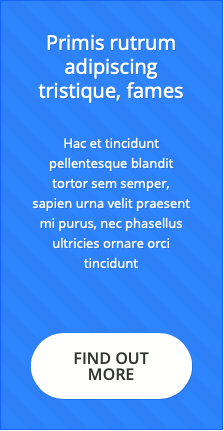
\includegraphics[scale=.5]{chamada-vertical-colorida-listrada}
    \caption{Chamada vertical colorida listrada}\label{RS0001:fig:chamada-vertical-colorida-listrada}
\end{figure}

\begin{code}
    \inputminted[label=chamada-vertical-colorida-listrada.html]{html}{../RS0001/anexos/chamada-vertical-colorida-listrada.html}
    \caption{Exemplo de chamada vertical colorida listrada}\label{RS0001:code:exemplo-chamada-vertical-colorida-listrada}
\end{code}


\subsubsection{Chamada vertical colorida com fundo listrado dinâmico}

Semelhante à ``Chamada vertical colorida com fundo listrado'' porém o fundo tem um efeito de visual de deslocamento (somente visível numa tela de computador).

\begin{figure}[!ht]
    \centering
    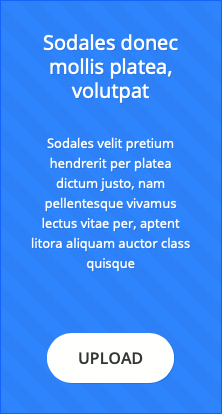
\includegraphics[scale=.5]{chamada-vertical-colorida-listrada-animada}
    \caption{Chamada vertical colorida listrada dinâmica}\label{RS0001:fig:chamada-vertical-colorida-listrada-animada}
\end{figure}

\begin{code}
    \inputminted[label=chamada-vertical-colorida-listrada-animada.html]{html}{../RS0001/anexos/chamada-vertical-colorida-listrada-animada.html}
    \caption{Exemplo de chamada vertical colorida listrada dinâmica}\label{RS0001:code:exemplo-chamada-vertical-colorida-listrada-animada}
\end{code}


\subsubsection{Chamada vertical longa com botão à esquerda}

\begin{figure}[!ht]
    \centering
    
\includegraphics[scale=.5]{chamada-vertical-longa-botao-esquerdo}
    \caption{Chamada vertical longa com botão à esquerda}\label{RS0001:fig:chamada-vertical-longa-botao-esquerdo}
\end{figure}

\begin{code}
    \inputminted[label=chamada-vertical-longa-botao-esquerdo.html]{html}{../RS0001/anexos/chamada-vertical-longa-botao-esquerdo.html}
    \caption{Exemplo de chamada vertical longa com botão à esquerda}\label{RS0001:code:exemplo-chamada-vertical-longa-botao-esquerdo}
\end{code}


\subsubsection{Chamada vertical longa com botão à direita destacado}

\begin{figure}[!ht]
    \centering
    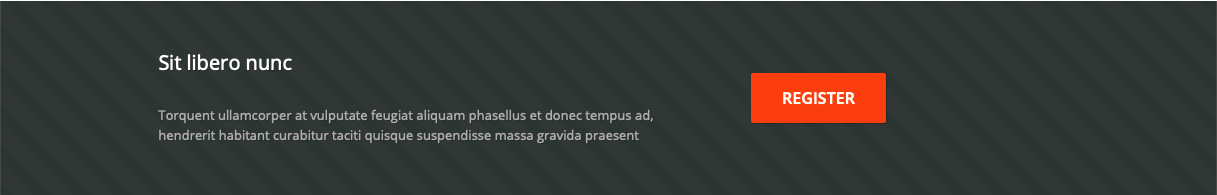
\includegraphics[scale=.5]{chamada-vertical-longa-botao-direito-destacado}
    \caption{Chamada vertical longa com botão à direita destacado}\label{RS0001:fig:chamada-vertical-longa-botao-direito-destacado}
\end{figure}

\begin{code}
    \inputminted[label=chamada-vertical-longa-botao-direito-destacado.html]{html}{../RS0001/anexos/chamada-vertical-longa-botao-direito-destacado.html}
    \caption{Exemplo de chamada vertical longa com botão à direita destacado}\label{RS0001:code:exemplo-chamada-vertical-longa-botao-direito-destacado}
\end{code}


\subsubsection{Chamada vertical longa com fundo listrado dinâmico botão central}

O fundo tem um efeito de visual de deslocamento (somente visível numa tela de computador).

\begin{figure}[!ht]
    \centering
    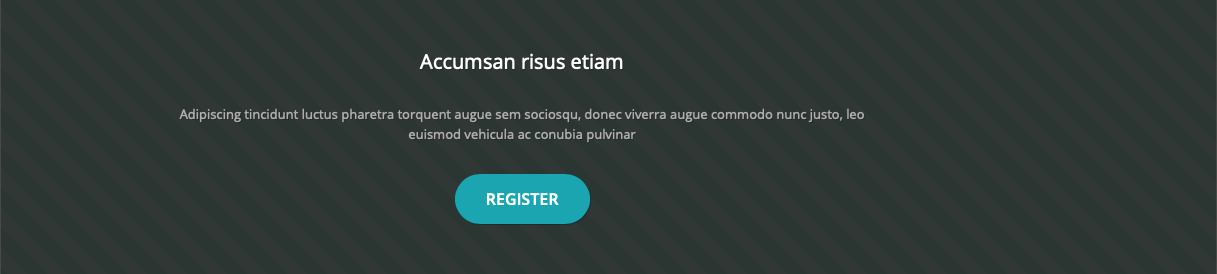
\includegraphics[scale=.5]{chamada-vertical-longa-botao-central}
    \caption{Chamada vertical longa com fundo listrado dinâmico botão central}\label{RS0001:fig:chamada-vertical-longa-botao-central}
\end{figure}

\begin{code}
    \inputminted[label=chamada-vertical-longa-botao-central.html]{html}{../RS0001/anexos/chamada-vertical-longa-botao-central.html}
    \caption{Exemplo de chamada vertical longa com fundo listrado dinâmico botão central}\label{RS0001:code:exemplo-chamada-vertical-longa-botao-central}
\end{code}

\subsection{Outros}


\subsubsection{Primeira letra em destaque}

Destacar a primeira letra de um texto.

\begin{figure}[!ht]
    \centering
    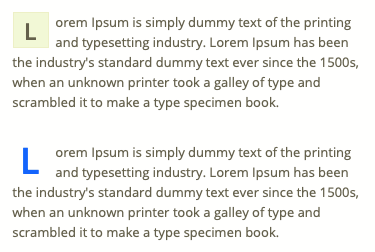
\includegraphics[scale=.5]{dropcaps}
    \caption{Primeira letra em destaque}\label{RS0001:fig:dropcaps}
\end{figure}

\begin{code}
    \inputminted[label=dropcaps.html]{html}{../RS0001/anexos/dropcaps.html}
    \caption{Exemplo de primeira letra em destaque}\label{RS0001:code:exemplo-dropcaps}
\end{code}


\subsubsection{Bloco de citação}

Bloco contendo uma citação, com nome do autor.

\begin{figure}[!ht]
    \centering
    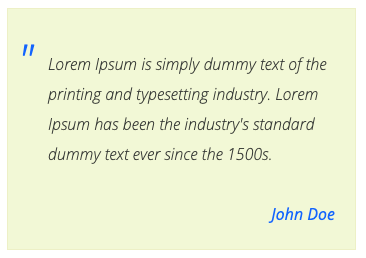
\includegraphics[scale=.5]{blockquote}
    \caption{Bloco de citação}\label{RS0001:fig:blockquote}
\end{figure}

\begin{code}
    \inputminted[label=blockquote.html]{html}{../RS0001/anexos/blockquote.html}
    \caption{Exemplo de citação}\label{RS0001:code:exemplo-blockquote}
\end{code}


\subsubsection{Listas}

Vários tipos diferentes de listas.

\begin{figure}[!ht]
    \centering
    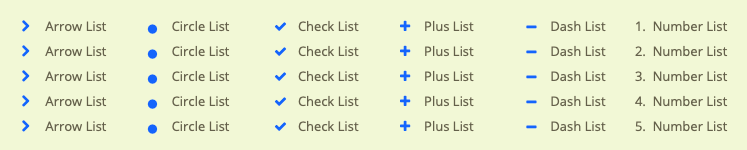
\includegraphics[scale=.5]{lists}
    \caption{Vários tipos de listas}\label{RS0001:fig:lists}
\end{figure}

\begin{code}
    \inputminted[label=lists.html]{html}{../RS0001/anexos/lists.html}
    \caption{Exemplos de listas}\label{RS0001:code:exemplo-lists}
\end{code}


\subsubsection{Tabelas}

Vários exemplos de tabelas.

\begin{figure}[!ht]
    \centering
    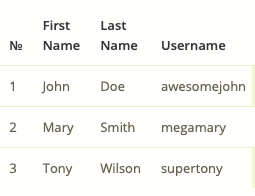
\includegraphics[scale=.5]{tables-1}
    \caption{Tabela simples}\label{RS0001:fig:tables-1}
\end{figure}

\begin{code}
    \inputminted[label=tables-1.html]{html}{../RS0001/anexos/tables-1.html}
    \caption{Exemplo de tabela simples}\label{RS0001:code:exemplo-tables}
\end{code}

\begin{figure}[!ht]
    \centering
    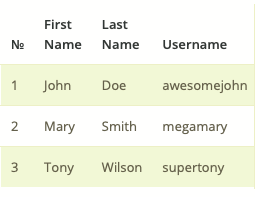
\includegraphics[scale=.5]{tables-2}
    \caption{Tabela com linhas de cores alternadas}\label{RS0001:fig:tables-2}
\end{figure}

\begin{code}
    \inputminted[label=tables-2.html]{html}{../RS0001/anexos/tables-2.html}
    \caption{Exemplo de tabela com linhas de cores alternadas}\label{RS0001:code:exemplo-tables-2}
\end{code}

\begin{figure}[!ht]
    \centering
    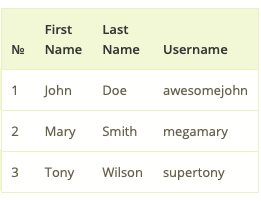
\includegraphics[scale=.5]{tables-3}
    \caption{Tabela com cabeçalho em destaque}\label{RS0001:fig:tables-3}
\end{figure}

\begin{code}
    \inputminted[label=tables-3.html]{html}{../RS0001/anexos/tables-3.html}
    \caption{Exemplo de tabela com cabeçalho em destaque}\label{RS0001:code:exemplo-tables-3}
\end{code}


\subsection{Organização do texto em colunas}

\subsubsection{Uma coluna}

\begin{figure}[!ht]
    \centering
    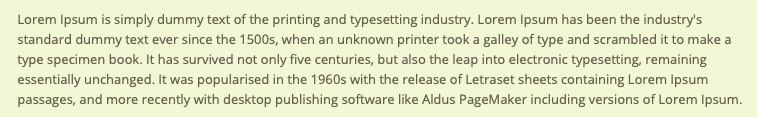
\includegraphics[scale=.5]{1-column}
    \caption{Uma coluna}\label{RS0001:fig:1-column}
\end{figure}

\begin{code}
    \inputminted[label=1-column.html]{html}{../RS0001/anexos/1-column.html}
    \caption{Exemplo de texto em uma coluna}\label{RS0001:code:exemplo-1-column}
\end{code}


\subsubsection{Duas colunas}

\begin{figure}[!ht]
    \centering
    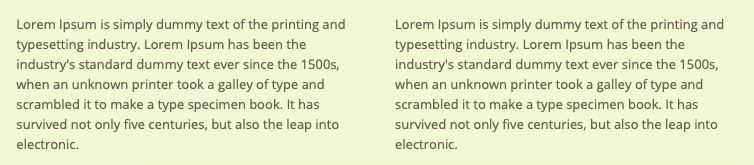
\includegraphics[scale=.5]{2-column}
    \caption{Duas colunas}\label{RS0001:fig:2-column}
\end{figure}

\begin{code}
    \inputminted[label=2-column.html]{html}{../RS0001/anexos/2-column.html}
    \caption{Exemplo de texto em duas colunas}\label{RS0001:code:exemplo-2-column}
\end{code}


\subsubsection{Três colunas}

\begin{figure}[!ht]
    \centering
    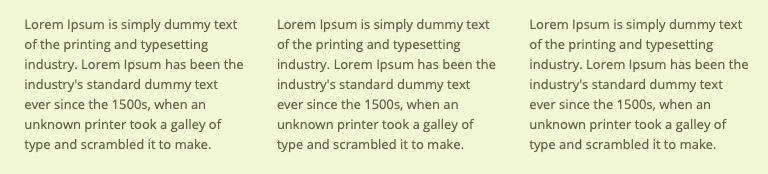
\includegraphics[scale=.5]{3-column}
    \caption{Três colunas}\label{RS0001:fig:3-column}
\end{figure}

\begin{code}
    \inputminted[label=3-column.html]{html}{../RS0001/anexos/3-column.html}
    \caption{Exemplo de texto em três colunas}\label{RS0001:code:exemplo-3-column}
\end{code}


\subsubsection{2/3 e 1/3 de espaço}

\begin{figure}[!ht]
    \centering
    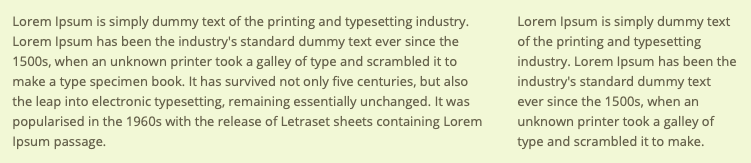
\includegraphics[scale=.5]{2-1-column}
    \caption{2/3 e 1/3 de espaço}\label{RS0001:fig:2-1-column}
\end{figure}

\begin{code}
    \inputminted[label=2-1-column.html]{html}{../RS0001/anexos/2-1-column.html}
    \caption{Exemplo de textos em 2/3 e 1/3 de espaço}\label{RS0001:code:exemplo-2-1-column}
\end{code}


\subsubsection{Quatro colunas}

\begin{figure}[!ht]
    \centering
    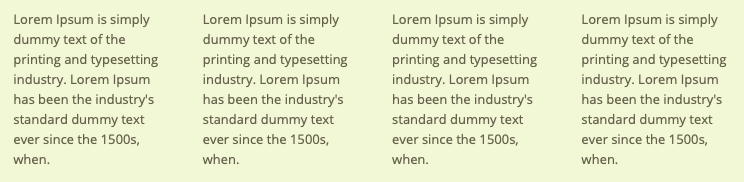
\includegraphics[scale=.5]{4-column}
    \caption{Quatro colunas}\label{RS0001:fig:4-column}
\end{figure}

\begin{code}
    \inputminted[label=1-4-column.html]{html}{../RS0001/anexos/4-column.html}
    \caption{Exemplo de texto em 4 colunas}\label{RS0001:code:exemplo-4-column}
\end{code}


\subsubsection{3/4 e 1/4 de espaço}

\begin{figure}[!ht]
    \centering
    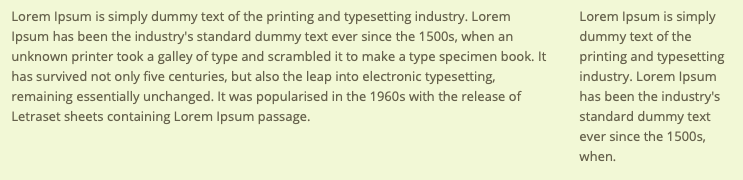
\includegraphics[scale=.5]{3-1-column}
    \caption{3/4 e 1/4 de espaço}\label{RS0001:fig:3-1-column}
\end{figure}

\begin{code}
    \inputminted[label=3-1-column.html]{html}{../RS0001/anexos/3-1-column.html}
    \caption{Exemplo de textos em 3/4 e 1/4 de espaço}\label{RS0001:code:exemplo-3-1-column}
\end{code}

\subsection{Referências}


\subsubsection{\textit{Links} para publicações, imagens, arquivos e páginas externas}

No editor \gls{WYSIWYG} é possível inserir \textit{links} para outras publicações, imagens, arquivos para os leitores do portal poderem fazer \textit{download} ou ligar para páginas externas.

Para cada tipo particular de \textit{link} é necessário seguir um format exato para que o elemento correto seja referenciado corretamente.

\begin{itemize}
    \item \textbf{Publicações} - as publicações dentro do próprio Portal do ITA possuem o formato \href{}{post/<slug>} onde o termo $<slug>$ se refere à um identificador criado para cada publicação à partir de seu título (veja na página da publicação o atributo $<slug>$ logo abaixo o título)
    \item \textbf{Imagem} - as imagens são referenciadas como \href{}{/image/<codigo-do-arquivo>} e são armazenadas como ``\textit{Archives}'' no repositório de documentos. Cada ``\textit{Archive}'' recebe um código identificador chamado $ID$ com letras e números de 24 dígitos que deve ser informado em $<codigo-do-arquivo>$
    \item \textbf{Arquivo} - do mesmo modo que as imagens, arquivos são referenciados como \href{}{/archive/<codigo-do-arquivo}
\end{itemize}